\subsection{Węzły pierwsze}

Liczby pierwsze znane z teorii liczb mają swój odpowiednik wśród węzłów.
Odpowiednik ten jest ściśle związany z operacją sumy spójnej, którą teraz zdefiniujemy.

\begin{definicja}
Niech $J$ i $K$ będą zorientowanymi węzłami.
Aby otrzymać ich sumę spójną, rozdzielamy je płaszczyzną i wybieramy gładką ścieżkę $\gamma \colon [0,1] \to \R^3$ z punktu $\gamma(0)$ w $J$ do $\gamma(1)$ w $K$, która nie przecina żadnego z diagramów.
Usuwamy krótkie łuki przy $\gamma(0)$ i $\gamma(1)$, po czym łączymy węzły ścieżką równoległą do $\gamma$.
\[
\begin{tikzpicture}[scale=0.05]
	% Figure Eight
	\path[ARC] (0,-10) .. controls (8,0) and (-8,0) .. (-8,8);
	\path[ARC] (-8,12) .. controls (-8,20) and (20,20) .. (1,1);
	\path[ARC] (5,10) .. controls (-30,16) and (-12,-22) .. (-3,-13);
	\path[ARC,decoration={markings, mark=at position .75 with {\arrow{<}}},postaction={decorate}]
		(-3,-3) .. controls (-7,-7) and (0,-15) .. (5,-15)
		.. controls (15,-15) and (19,7) .. (10,9);
	\node at (0,-20) {$J$}; 
	% Trefoil
	\path[ARC] (50+0,10) .. controls (50+10,0) and (50+-10,0) .. (50+0,-10);
	\path[ARC] (50+-1.5,1.5) .. controls (50+-6,6) and (50+-3,17) .. (50+10,12)
		.. controls (50+23,7) and (50+15,-20)  .. (50+3,-13);
	\path[ARC,decoration={markings, mark=at position .6 with {\arrow{>}}},postaction={decorate}]
		 (50+1.5,-1.5) .. controls (50+6,-6) and (50+3,-17) .. (50+-10,-12)
		.. controls (50+-23,-7) and (50+-15,20)  .. (50+-3,13);
	\node at (0,-20) {$J$};
	\node at (50,-20) {$K$};
\end{tikzpicture}
\begin{tikzpicture}[scale=0.05]
	%Figure-eight
	\path[ARC] (0,-10) .. controls (8,0) and (-8,0) .. (-8,8);
	\path[ARC]
		(-8,12) .. controls (-8,20) and (20,20) .. (1,1);
	\path[ARC] (5,10) .. controls (-30,16) and (-12,-22) .. (-3,-13);
	\path[ARC] (-3,-3) .. controls (-7,-7) and (0,-15) .. (5,-15);
	%trefoil
	\path[ARC] (50+0,10) .. controls (50+10,0) and (50+-10,0) .. (50+0,-10);
	\path[ARC] (50+-1.5,1.5) .. controls (50+-6,6) and (50+-3,17) .. (50+10,12)
		.. controls (50+23,7) and (50+15,-20)  .. (50+3,-13);
	% Bottom connector
	\path[ARC,decoration={markings, mark=at position .65 with {\arrow{>}}},postaction={decorate}]
		(50+1.5,-1.5) .. controls (50+12,-15) and (50+-14,-18) .. (50+-16,-5)--
		(15,-5) .. controls (15,-10) and (10,-15) .. (5,-15);
	% Top connector
	\path[ARC,decoration={markings, mark=at position .4 with {\arrow{>}}},postaction={decorate}]
		(10,9) .. controls (15,8) and (15,3)  .. (15,0)--
		(50+-16.5,0) .. controls (50+-16.5,10) and (50+-11,17) .. (50+-3,13);
	\node at (25,-20) {$J\#K$};
\end{tikzpicture}\]

\end{definicja}

Operacja sumy spójnej określona jest jedynie dla zorientowanych węzłów, ponieważ bez orientacji istnieje drugi, być może nierównoważny sposób na połączenie diagramów.
Nie ma ona też sensu dla splotów, nawet zorientowanych, gdyż nie istnieje dla nich kanoniczny sposób na wybór, które składowe należałoby ze sobą połączyć.

\begin{twierdzenie}
Niech $J, K$ będą zorientowanymi węzłami.
Ich suma spójna jest dobrze określona i zależy jedynie od klas równoważności, a nie samych węzłów.
\end{twierdzenie}

\begin{proof}(Szkic)
Załóżmy, że mamy dane węzły $J, K$ oraz ścieżki $\gamma$, $\delta$, których używamy do stworzenia sumy $J\# K$.
Wykonujemy następujące kroki.
\begin{enumerate}
\item Kurczymy $K$.
\item Przesuwamy $K$ wzdłuż $\gamma$ tak, by leżało blisko $\gamma(0)$.
\item Przesuwamy $K$ wzdłuż $J$ od $\gamma(0)$ do $\delta(0)$.
\item Odwracamy dwa pierwsze kroki z $\delta$ w miejscu $\gamma$.\qedhere
\end{enumerate}
\end{proof}



\begin{twierdzenie}
Suma spójna jest działaniem łącznym i przemiennym.
Niewęzeł $\NieWezel$ jest jego elementem neutralnym.
\end{twierdzenie}

\begin{proof}
Przedstawmy węzły $I, J, K$ w następujący sposób:
\[\begin{tikzpicture}[scale=0.08]
%	\clip (-21,-16) rectangle (21,16);
	\path[ARC] (-50,0) rectangle (-40,-10);
	\path[ARC,-<-] (-40,-2) .. controls (-35,-2) and (-35,-8) .. (-40,-8);
	\node () at (-45,-5) {$I$};

	\path[TEXTARC, blue,->-] (-35,-5) -- node[auto] () {$\gamma$} (-25,-5);

	\path[ARC] (-20,0) rectangle (-10,-10);
	\path[ARC,->-] (-20,-2) .. controls (-25,-2) and (-25,-8) .. (-20,-8);
	\path[ARC,-<-] (-10,-2) .. controls (-5,-2) and (-5,-8) .. (-10,-8);
	\node () at (-15,-5) {$J$};
	
	\path[TEXTARC, blue,->-] (-5,-5) -- node[auto] () {$\delta$} (5,-5);
	
	\path[ARC] (10,0) rectangle (20,-10);
	\path[ARC,->-] (10,-2) .. controls (5,-2) and (5,-8) .. (10,-8);
	\node () at (15,-5) {$K$};
\end{tikzpicture}\]
Tworzymy sumy $I\#(-)$ przy użyciu $\gamma$, $(-)\#K$ przy użyciu $\delta$.
Wtedy $(I\#J)\#K$ oraz $I\#(J\#K)$ są dane przez
\[\begin{tikzpicture}[scale=0.08]
%	\clip (-21,-16) rectangle (21,16);
	\path[ARC] (-50,0) rectangle (-40,-10);
	\node () at (-45,-5) {$I$};
	\path[ARC] (-20,0) rectangle (-10,-10);
	\node () at (-15,-5) {$J$};
	\path[ARC] (10,0) rectangle (20,-10);
	\node () at (15,-5) {$K$};

	\path[ARC,-<-] (-40,-2) -- (-20,-2);
	\path[ARC,->-] (-40,-8) -- (-20,-8);

	\path[ARC,-<-] (-10,-2) -- (10,-2);
	\path[ARC,->-] (-10,-8) -- (10,-8);
\end{tikzpicture},\]
a przez to równoważne.

Do pokazania przemienności wystarcza obserwacja, że jeżeli $J \# K$ powstaje przy użyciu łuku $\gamma$, to $K \# J$ otrzymujemy biorąc odwrotność $\gamma$ (ten sam łuk o przeciwnej orientacji).

Przedstawmy wreszcie $K$ i $\NieWezel$ tak, jak po lewej stronie i stwórzmy sumę $K \# \NieWezel$ łukiem $\gamma$.
Wtedy $K\#\NieWezel$ jest równoważny z prawym węzłem, a ten z samym $K$, co kończy dowód.
\[\begin{tikzpicture}[scale=0.08]
%	\clip (-21,-16) rectangle (21,16);
	\path[ARC] (-50,0) rectangle (-40,-10);
	\path[ARC,-<-] (-40,-2) .. controls (-35,-2) and (-35,-8) .. (-40,-8);
	\node () at (-45,-5) {$K$};

	\path[TEXTARC, blue,->-] (-35,-5) -- node[auto] () {$\gamma$} (-25,-5);

	\path[ARC,->-] (-19,-5) circle (5);
\end{tikzpicture}
\qquad\qquad\qquad\qquad
\begin{tikzpicture}[scale=0.12]
%	\clip (-21,-16) rectangle (21,16);
	\path[ARC] (-50,0) rectangle (-40,-10);
	\node () at (-45,-5) {$K$};
	
	\path[ARC,->-] (-19,-5) circle (5);
	\path[fill=white] (-19,-2) rectangle (-30,-8);

	\path[ARC,-<-] (-40,-2) -- (-22.8,-2);
	\path[ARC,->-] (-40,-8) -- (-22.8,-8);	
\end{tikzpicture}
\qedhere
\]
\end{proof}

Możemy przejść do definicji węzłów pierwszych.

\begin{definicja}
Zorientowany węzeł $J$ jest pierwszy, jeżeli nie jest niewęzłem i nie można zapisać go jako suma spójna dwóch nietrywialnych węzłów.
\end{definicja}

Tabela węzłów zawiera wszystkie węzły pierwsze, przy czym lustra i odwrotności są w niej pominięte.
Jest ona uporządkowana według indeksu krzyżującego: najmniejszej liczby skrzyżowań, jaką można osiągnąć na diagramie węzła.
Na końcu tego dokumentu przedstawione są węzły o mniej niż ośmiu skrzyżowaniach.
Atlas węzłów
\begin{itemize}
\item \url{http://katlas.math.toronto.edu/wiki/The_Rolfsen_Knot_Table}
\end{itemize}
podaje więcej węzłów: o mniej niż jedenastu skrzyżowaniach.
Pozwala także na sprawdzenie różnych niezmienników.

W tym miejscu pojawia się pytanie, czy niewęzeł nie jest być może złożony.
Gdyby tak rzeczywiście było, każdy węzeł okazałby się złożony, jako suma spójna siebie z niewęzłem.
Na szczęście przy pomocy powierzchni (Seiferta) można pokazać, że niewęzeł nie powstaje z dwóch nietrywialnych węzłów przez wzięcie sumy spójnej.

Ze względu na niedostatecznie rozwinięty aparat matematyczny nie możemy podać dowodu następującego faktu, analogonu zasadniczego twierdzenia arytmetyki.

\begin{twierdzenie}[Schubert, 1949]
Każdy węzeł rozkłada się jednoznacznie na węzły pierwsze (z dokładnością do kolejności składników).
\end{twierdzenie}

Czy węzłów pierwszych jest nieskończenie wiele?
Tak, potrafimy nawet oszacować ich liczbę.
W roku 1987 C. Ernst wraz z D. Sumnersem w oparciu na wynikach Kauffmana, Murasugiego oraz Thistlethwaite'a dotyczących węzłów alternujących pokazali, że różnych węzłów pierwszych o $n$ skrzyżowaniach jest co najmniej $\frac 1 3 (2^{n- 2} - 1)$ dla $n \ge 4$, przy czym węzły lustrzane traktowane są jako różne.
Niedawno D. Welsh pokazał, że liczba takich węzłów jest ograniczona z góry przez funkcję wykładniczą od $n$.

% Przykładem nieskończonej rodziny węzłów, które są parami różne, są węzły torusowe.

W roku 1985 M. Scharleman rozwiązał otwarty od ponad stu lat problem wiążący pierwszość z liczbą rozsupłującą\footnote{unknotting number}: jeżeli odwrócenie dokładnie jednego skrzyżowania wystarcza do zmiany węzła w niewęzeł, to jest on pierwszy.

\begin{figure}[!ht]
\centering
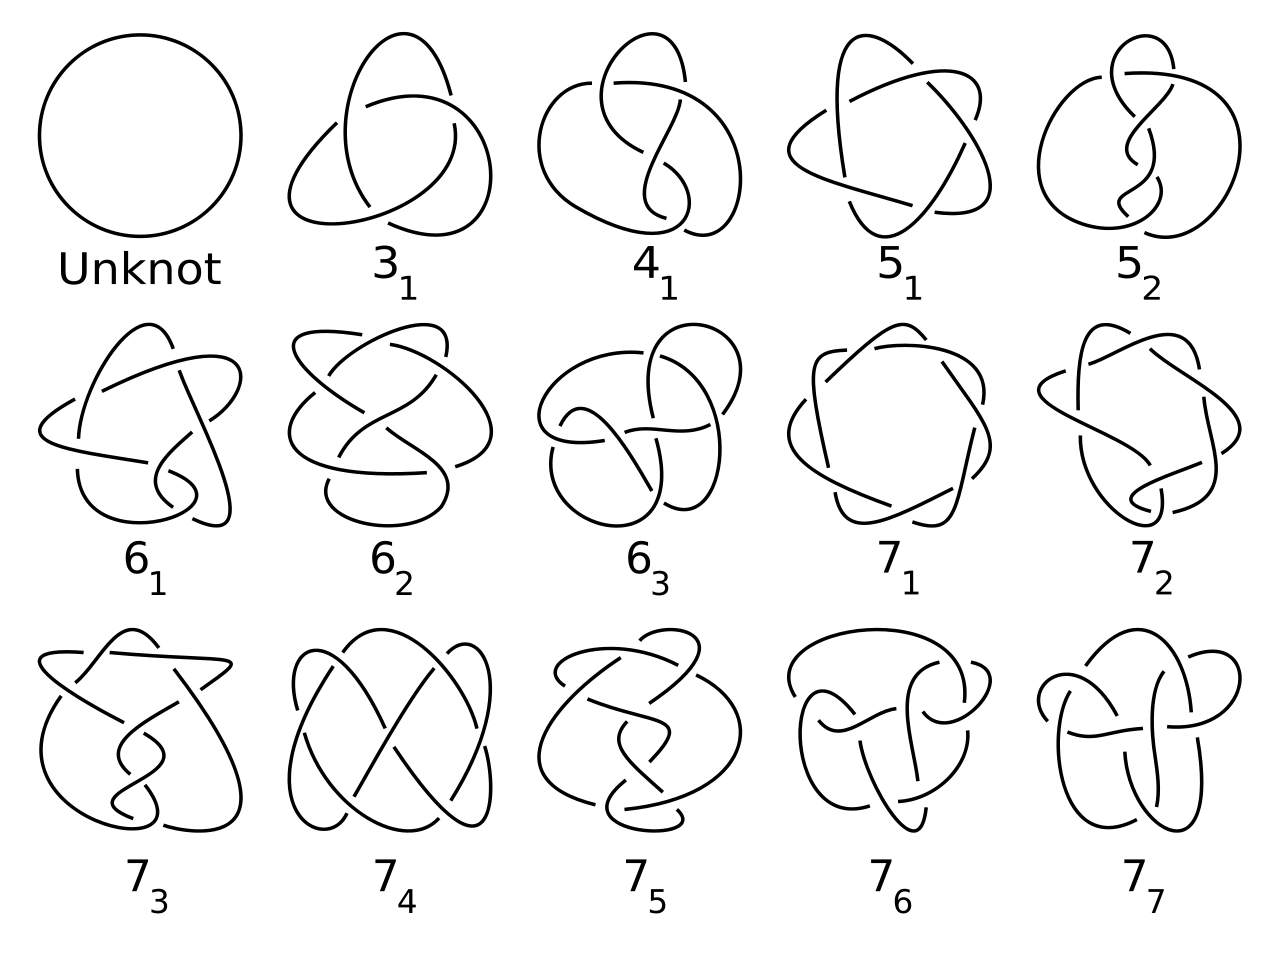
\includegraphics[scale=0.25]{4/knoty.png}
\caption{Niewęzeł i węzły pierwsze o mniej niż 8 skrzyżowaniach.}
\end{figure}